\subsection{Schallwellen}
Schallwellen sind Druckwellen und können sich daher nur in Medien ausbreiten. Sie sind longitudinale Wellen, die durch
\begin{align}
	p(x, t) = p_0 + v_0 Z \cos(\omega t-kx)
\end{align}
beschrieben werden. Der Druck $p$ schwankt demnach mit einer Amplitude von $v_0Z$ um den \grqq Grunddruck\grqq\ $p_0$. Die akustische Impedanz $Z$ ist dabei eine wichtige Materialeigenschaft, die das Produkt der Dichte des Mediums $\rho$ und der Schallgeschwindigkeit im Medium
\begin{align}
	c = \sqrt{\frac{A}{\rho}}
\end{align}
ist. Bei Flüssigkeiten ist die Konstante $A$ das Inverse Kompressibilität $\kappa$, bei Festkörpern ist $A$ das Elastizitätsmodul $E$. \\
Wird die Ausbreitung im Festkörper genauer betrachtet, kann festgestellt werden, dass die hier auch ein transversaler Anteil vorhanden ist. Das bedeutet, dass die Ausbreitung Richtungsabhängig ist.
Da es sich bei Druckänderungen um Teilchenbewegungen handelt, kommt es zu Energieverlusten (durch Umwandlung in Wärme). Das bedeutet, dass die Intensität bei Ausbreitung in $x$-Richtung exponentiell abfällt
\begin{align}
	I(x) = I_0 e^{-\alpha x} \ ,\qquad \alpha>0 \ .
\end{align}
Da der Absorptionskoeffizient $\alpha$ von Luft beispielsweise sehr groß ist, wird üblicherweise ein Kontaktmittel zwischen Schallgeber und Material verwendet. So kann der Energieverlust verringert werden. Nicht zu verhindern ist die Reflexion an einer Grenzfläche zwischen einem Medium mit akustischer Impedanz $Z_1$ und einem zweiten Medium mit $Z_2$. Das Verhältnis von einfallender und reflektierter Welle wird durch den Reflexionskoeffizienten
\begin{align}
	R = \left(\frac{Z_1-Z_2}{Z_1+Z_2}\right)^2
\end{align}
beschrieben. Der transmittiert Anteil ist dann $T = 1-R$.
\subsection{Verfahren der Ultraschallechographie}
Um Medien mit Hilfe von Ultraschall zu untersuchen wird meistens eine der folgenden Methoden verwendet.
\subsubsection*{Durchschallungsverfahren (Abbildung \ref{fig:Durchschall})}
Ein Ultraschallsender sendet einen Impuls aus. Die Welle breitet sich durch das Medium aus und wird danach von einem Empfänger detektiert. Befindet sich beispielsweise ein Fremdkörper im Material wird das vom Empfänger in Form einer abgeschwächten Intensität registriert.
\subsubsection*{Impuls-Echo-Verfahren (Abbildung \ref{fig:ImpulsEcho})}
Auch hier sendet der Ultraschallsender einen Impuls aus. Die Schallwelle propagiert im Medium. Hinter dem Medium sollte ein Material mit möglichst kleiner akustischer Impedanz sein, sodass ein Großteil der Welle reflektiert wird. Die Welle läuft zurück und wird vom Sender, der gleichzeitig Empfänger ist, detektiert. Ein Fremdkörper wird dadurch bemerkt, dass die hinlaufende Welle schon an ebendiesem reflektiert wird und somit vor der bis zum Ende gelaufenen Welle am Empfänger ankommt.
\begin{figure}[h!]
	\centering
	\begin{subfigure}{.5\textwidth}
		\centering
		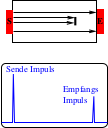
\includegraphics[width=.4\textwidth]{Durchschallung.png}
		\caption{Durchschallungsverfahren}
		\label{fig:Durchschall}
	\end{subfigure}%
	\begin{subfigure}{.5\textwidth}
		\centering
		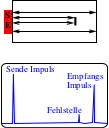
\includegraphics[width=.4\textwidth]{ImpulsEcho.png}
		\caption{Impuls-Echo-Verfahren}
		\label{fig:ImpulsEcho}
	\end{subfigure}
	\caption{Prinzipielle Darstellung der Verfahren, mit denen Materialien mit Hilfe von Ultraschall untersucht werden können \cite{\V}}
	\label{fig:test}
\end{figure} \\
Bei beiden Verfahren kann die Länge des untersuchten Körpers mit Hilfe von
\begin{align}
	L = c \cdot \Delta t
\end{align}
bestimmt werden, wenn die Schallgeschwindigkeit des Mediums bekannt ist. Wichtig ist dabei, dass die Durchlaufzeit $\Delta t$ die Zeit ist, die vergeht, bis die Strecke $L$ zurückgelegt wird, beim Impuls-Echo-Verfahren wird in der gemessenen Zeit allerdings die Strecke $2L$ zurückgelegt.

\subsection{Darstellung der Signale}
\subsubsection*{A-Scan}
Im A-Scan wird das reflektierte Signal als Funktion der Zeit oder der Eindringtiefe dargestellt. Für letzteres muss die Schallgeschwindigkeit im untersuchten Objekt bekannt sein.
\subsubsection*{B-Scan}
Bei einem B-Scan wird ein Objekt in zwei Dimensionen untersucht. Mit Hilfe verschiedener Farben wird die Intensität des reflektierten Signals an jedem Ort dargestellt.
\subsubsection*{TM-Scan}
Der Time-Motion-Scan ist dem B-Scan sehr ähnlich. Allerdings liegt der Fokus hier nicht auf der räumlichen Situation, sondern auf der zeitlichen Veränderung des reflektierten Signals.
